\documentclass[12pt]{artikel3}                  % I need a font of 12 for the proposal.
\linespread{1.2}                                % Not sure why we need this here.
\usepackage{fullpage, setspace, graphicx}       % What does the full page library do?
\usepackage{mathtools, amsfonts}                % Mathtools are understandable, and so are the amsfonts that are being used.
\usepackage[margin=1in]{geometry}
\usepackage{newcent}                            % Why do I need the newcent package or what it does?
\usepackage{url}                                % If I am including URL in any place, I will need this package.
\usepackage{cite}                               % Need this for citing of the various formats.
\usepackage{hyperref}
\usepackage{algorithm}
\usepackage{algpseudocode}

\begin{document}
\begin{titlepage}
\begin{center}

\textsc{\LARGE }\\[0.2cm]
\textsc{\LARGE }\\[0.2cm]
\textsc{\LARGE }\\[1.2cm]

\textsc{\Large Master's Project Proposal}\\[1cm]

\large{Soham Sadhu}\\
\large{Department of Computer Science}\\
\large{Rochester Institute of Technology}\\
\large{Rochester, NY 14623}\\
\large{sxs9174@rit.edu}\\[0.5cm]

{\large \today}\\[1cm]

\begin{tabular}{l l r}
    Chair: & Prof. Stanis{\l}aw Radziszowski & spr@cs.rit.edu\\[1.5cm] \hline
    \multicolumn{3}{c}{signature \hspace{6cm} date}\\[1cm]
    Reader: & Prof. Leon Reznik & lr@cs.rit.edu\\[1.5cm] \hline
    \multicolumn{3}{c}{signature \hspace{6cm} date}\\[1cm]
    Observer: & & \\[1.5cm] \hline
    \multicolumn{3}{c}{signature \hspace{6cm} date}\\[1cm]
\end{tabular}


\vfill

\end{center}
\end{titlepage}

\begin{center}
\parbox{350pt}{
  \begin{center}\textsc{Abstract}\end{center}
  \vspace{0.5cm}
  \href{"http://en.wikipedia.org/wiki/Cryptographic\_hash\_function\#Applications"}
  {Message integrity, password authentication} over the Internet relies on cryptographic hash
  function. Due to importance of hash function usage in everyday computing, standards for hashing 
  algorithm and their bit size have been released by NIST \cite{00037} which are 
  denoted by nomenclature Standard Hashing Algorithm (SHA).

  Due to advances in cryptanalysis of SHA-2, NIST announced a competition in November 2007, 
  to choose SHA-3. In October 2012, the winner was selected to be \href{"http://keccak.noekeon.org/"}
  {Keccak} amongst 64 submissions \cite{00038, 00039}. All the submissions were open to public scrutiny, 
  and underwent intensive third party cryptanalysis, before the winner was selected. 
  Keccak was chosen for its flexibility, efficient and elegant implementation, and large security 
  margin \cite{00040}.

  All algorithms submitted to competition have undergone public scrutiny. And other four finalist in 
  the competition were almost equivalent to Keccak, in attributes of security margin and implementation.
  In this project, I will compare Keccak with two other SHA-3 finalists, \href{"https://131002.net/blake/"}
  {BLAKE}, and \href{"http://www.groestl.info/"}{Gr{\o}stl} on ease of finding near collisions, using
  \href{"http://en.wikipedia.org/wiki/Simulated\_annealing"}{simulated annealing} and 
  \href{"http://en.wikipedia.org/wiki/Tabu\_search"}{tabu search}.
  
  When Hamming weight of two message digests XORed, which are obtained from same hash function, with two
  different messages with same chaining value. Evaluate to a number, which is equal to or less than 
  ${1/4}^{th}$ of the number of bits in the message digest, then it is considered as a near collision.
  
  Tabu search and simulated annealing, can be categorised as generic attacks on a hash function. That is
  these methods of attacking hash functions are design agnostic. At present, it is computationally 
  infeasible to break the above mentioned hash functions, but the reduced versions of these can be 
  subjected to attacks for near collisions. I will implement the hash functions Keccak, BLAKE and
  Gr{\o}stl. Then subject them to hill climbing, simulated annealing, tabu search, and random selection 
  of chaining value from a sample; for finding near collisions.
  
  The aim is to see, if tabu search and simulated annealing are better at finding near collisions, than
  hill climbing \cite{00029}. And by what margin, are these algorithms better than a naive random search
  for near collisions.
}
\end{center}

\clearpage

\section{Problem Statement}

\subsection{Hash Functions}
A cryptographic hash function, is an algorithm capable of intaking arbitrarily long input string, and
output a fixed size string, often called a message digest. The message digest for two strings even 
differing by a single bit should ideally be completely different. And no two different input messages
known, should have the same hash value. This property enables us to fingerprint a message. Following 
are the properties of an ideal hash function\cite{00005}.
  
1. {\bf Preimage resistance}
\begin{center}
  \framebox
  {
    \parbox{350pt}
    {
      \centering \textsc{Preimage} \\
      {\bf Given:} A hash function $h : \mathcal{X} \to \mathcal{Y}$ and an element $y \in \mathcal{Y}$. \\
      {\bf Find:} $x \in \mathcal{X}$ such that $h(x) = y$. 
    }
  }
\end{center}
\vspace{4mm}
If the preimage problem for a hash function cannot be efficiently solved, then it is preimage resistant.
That is the hash function is one way, or rather it is difficult to find the input, given the output alone.

2. {\bf Second preimage resistance}
\begin{center}
  \framebox
  {
    \parbox{350pt}
    {
      \centering \textsc{Second preimage} \\
      {\bf Given:} A hash function $h : \mathcal{X} \to \mathcal{Y}$ and an element $x \in \mathcal{X}$. \\
      {\bf Find:} $x' \in \mathcal{X}$ such that $x' \neq x$ and $h(x) = h(x')$. 
    }
  }
\end{center}
\vspace{4mm}

A hash function for which a different input given another input, that compute to same hash cannot be found 
easily, is called as having second preimage resistance.

3. {\bf Collision resistance}
\begin{center}
  \framebox
  {
    \parbox{350pt}
    {
      \centering \textsc{Collision} \\
      {\bf Given:} A hash function $h : \mathcal{X} \to \mathcal{Y}$.  \\
      {\bf Find:} $x, x' \in \mathcal{X}$ such that $x' \neq x$ and $h(x') = h(x)$. 
    }
  }
\end{center}
\vspace{4mm}

Collision problem states that, can two different input strings be found, such that they hash to the same
value given the same hash function. A hash function is collision resistant, if it is computationally
infeasible to find two different values hashing to same value.

\subsection{Standards and NIST Competition}

Since hash functions can fingerprint any data, they find wide applications in computer security. Thus there
needs to be a standard for implemenation and application of hash function, which is provided by National Institute
of Standards and Technology(NIST)\cite{00037}. SHA-0 was initially proposed by National Security Agency(NSA), as 
a standardised hashing algorithm in 1993. It was later standardised by NIST. In 1995 SHA-0 was replaced by SHA-1 
designed by NSA \cite{00006, 00007}. SHA-2 was designed by NSA, and released in 2001 by NIST. It is basically a 
family of hash functions consisting of SHA-224, SHA-256, SHA-384, SHA-512. The number suffix after the SHA acronym, 
indicates the bit length, of the output of that hash function. Although SHA-2 family of algorithms were influenced
by SHA-1 design, but the attacks on SHA-1 have not been successfully extended to SHA-2.

In response to advances made in cryptanalysis of SHA-2. NIST announced a public competition on November 2007,
for a new cryptographic hash algorithm, that would be SHA-3. 51 candidates from 64 submissions for first round 
of competition were announced in December, 2008 \cite{00039}. In October, 2012 NIST announced the winner of the 
competition to be Keccak, amongst the other four finalist, which were BLAKE, Gr{\o}stl, JH and Skein. Keccak 
was chosen for its' large security margin, efficient hardware implementation, and flexibility \cite{00040}.

\subsection{Objective}

The arguments for choosing Keccak as SHA-3 are strong. However, other 4 finalists, have similar strong claims 
to security margin; one of the attributes on which Keccak was chosen. All the finalists have gone through 
public scrutiny, and have shown resistance, to a number of attacks.

\vspace{3mm}
\begin{center}
  \framebox
  {
    \parbox{400pt}
    {
      \centering \textsc{Hypothesis} \\
      \begin{itemize}
      \item Reduced state Keccak, has better resistance to near collisions than BLAKE and Gr{\o}stl. For the
      attack algorithms hill climbing, simulated annealing, tabu search and random selection.
      \item Simulated annealing and tabu search, are better at finding near collisions compared to hill 
      climbing and random selection.
      \end{itemize}
      %Reduced round Keccak, will have better resistance to near collisions found by tabu search and simulated
      %annnealing, compared to reduced round BLAKE and Gr{\o}stl.
    }
  }
\end{center}
\vspace{3mm}

The aim of the project is to study reduced version of Keccak holds security margin, comparable to reduced
versions of BLAKE and Gr{\o}stl. This will be done by comparing the amount of computational resources required
to find near collisions for two different messages with same chaining value; using simulated annealing, tabu
search, hill climbing and random sampling of chaining values. When Hamming weight of two message digests XORed, 
which are obtained from same hash function, with two different messages with same chaining value. Evaluate to 
a number, which is equal to or less than ${1/4}^{th}$ of the number of bits in the message digest, then it is
considered as a near collision. The collected data will also be studied, to compare the effectiveness of
the 4 attack algorithms; in finding near collisions.
 
\clearpage

\section{Background}

\subsection{Gr{\o}stl}

Gr{\o}stl is collection of hash functions which produce digest size, ranging from 1 to 64 bytes. The variant of
Gr{\o}stl that returns a message digest of size n, is called Gr{\o}stl-n. Gr{\o}stl is an iterated hash function, 
with two compression functions named $P$ and $Q$. The input is padded and then split into $l$-bit message blocks
$m_{1}$,$\ldots$, $m_{t}$, and each message block is processed sequentially. The initial $l$-bit chaining value 
$h_{0}$ = iv is defined, and the blocks $m_{i}$ are processed as $ h_{i}\gets f(h_{i-1}, m_{i})$ for i = 1,$\ldots$,
t. For variants up to 256 bits output, size of $l$ is 256 bits. And for digest sizes larger than 256 bits, $l$ 
is 1024 bits. After the last message block is processed, the last chaining value output is sent through a 
$\Omega$ function, to get the hash output $H(M)$ \cite{00019}. 

\begin{center}$H(M) = \Omega(h_{t}),$\end{center}

The function $f$, is composed of two $l$-bit permutations called $P$ and $Q$, which is defined as follows.

\begin{center}$f(h, m) = P(h \oplus m) \oplus Q(m) \oplus h.$\end{center}

The function $\Omega$, consists of a $trunc_{n}(x)$ that outputs only the trailing n bits of input $x$.
\begin{center}$\Omega(x) = trunc_{n}( P(x) \oplus x ).$\end{center}

In order to fit the varying input length message to the block sizes of $l$ padding is defined. First bit '1' is
appended, then $ w = -N - 65 \mod l $ 0 bits are appended; where N is the length of the original message. And then
a 64 bit representation of $(N + w + 65) / l $ is padded at the end.

There are two variations for $P$ and $Q$ permutations, one each for the digest size lower and higher than 256 bits. There
are four round transformations, that compose a round R. The permutation consists of a number of rounds R, and can be
represented as 

\begin{center} R = MixBytes $\circ$ ShiftBytes $\circ$ SubBytes $\circ$ AddRoundConstant \end{center}

The transformations SubBytes and MixBytes are same for all transformation while, ShiftBytes and AddRoundConstant differ
for each of the transformations. The transformations operate on matrix of bytes, with the permutation of lower size
digest having matrix of 8 rows and 8 columns, while that for larger variant is of 16 columns and 8 rows. The number of
rounds for digest sizes upto 256 bits are 10. For digest sizes higher than that, number of rounds are 14. The individual
components of each round for $P$ and $Q$ are described below.

{\bf AddRoundConstant:} transformation round XOR a round dependant constant to the state matrix say $A$. It is 
represented as $A \gets A \oplus C[i]$, where $C[i]$ is the round constant in round $i$.

{\bf SubBytes:} substitutes each byte in state by value from S-box. Say $a_{i,j}$ a element in row $i$ and column $j$
of the state matrix, then the transformation done is $a_{i,j} \gets S( a_{i,j}),  0 \leq i < 8, 0 \leq j < v.$

{\bf ShiftBytes:} transformation cyclically shifts the bytes in a row to left by that number. Let list vector 
of a number denote the shift, with the index of the element indicating the row. The vector representation for
$P_{512}$ = [0, 1, 2, 3, 4, 5, 6, 7] and $Q_{512}$ = [1, 3, 5, 7, 0, 2, 4, 6]. Those for the larger permutation 
are $P_{1024}$ = [0, 1, 2, 3, 4, 5, 6, 11] and $Q_{1024}$ = [1, 3, 5, 11, 0, 2, 4, 6].

{\bf MixBytes:} transformation, multiplies each column of the state matrix $A$, by a constant 8 $\times$ 8 matrix
$B$. The transformation, can be shown as $ A \gets B \times A$. The matrix B, can be seen as a finite field over 
$\mathbb{F}_{256}$. This finite field is defined over $\mathbb{F}_{2}$ by the irreducible polynomial 
$x^{8} \oplus x^{4} \oplus x^{3} \oplus x \oplus 1$.

\subsection{BLAKE}

BLAKE\cite{00002} hash function is built on HAIFA (HAsh Iterative FrAmework) structure \cite{00020} which is an improved
version of Merkle-Damg\.{a}rd function. BLAKE has 4 variations of the algorithm that can give only 4 different digest
lengths. The construction takes in 4 inputs, one message; two a salt, that makes function that parameter specific; and
three a counter, which is count of all the bits hashed till then; and lastly a chaining value which is input of the previous
operation or initial value in case of hash initiation. The compression function is composed of a 4 $\times$ 4 matrix of words.
Where one word is equal to 32 bits for BLAKE-256 variant, while 64 bit for variant BLAKE-512.

\begin{table}[h]
  \begin{center}
    \begin{tabular}{ c l } \hline
      Symbol                 & Meaning \\ \hline
      $\gets$                    & variable assignment \\
      $+$                    & addition modulo $2^{32}$ or (modulo $2^{64}$) \\
      $\gg k$                  & rotate k bits to least significant bits \\
      $\ll k$                  & rotate k bits to most significant bits \\
      $\langle l \rangle_{k}$ & encoding of integer $l$ over $k$ bits \\ \hline
    \end{tabular}
    \caption{Convention of symbols used in BLAKE algorithm}
  \end{center}
\end{table}

\subsubsection{ BLAKE-256 }

The compression function takes following as input
\begin{itemize}
  \item a chaining value of $h = h_{0},\dots, h_{7}$
  \item a message block $m = m_{0},\dots, m_{15}$
  \item a salt $s = s_{0},\dots, s_{3}$
  \item a counter $t = t_{0}, t_{1}$
\end{itemize}
These four inputs of 30 words or 120 bytes, are processed as $h' = compress(h, m, s, t)$ to provide a new
chain value of 8 words.

{\bf Compression function}

\begin{itemize}
\item {\bf Constants}
  \begin{table}[h]
    \begin{center}
      \begin{tabular}{ *{4}{c}}
        $IV_{0}$ = 6A09E667 & $IV_{1}$ = BB67AE85 & $IV_{2}$ = 3C6EF372 & $IV_{3}$ = A54FF53A \\
        $IV_{4}$ = 510E527F & $IV_{5}$ = 9B05688C & $IV_{6}$ = 1F83D9AB & $IV_{7}$ = 5BE0CD19 \\
      \end{tabular}
      \caption{Initial values which become the chaining value for the first message block}
    \end{center}
  \end{table}
  
  \begin{table}[h]
    \begin{align*}
         {\tt c_{0}}  &= {\tt 243F6A88} & {\tt c_{1}}  &= {\tt 85A308D3} & {\tt c_{2}}  &= {\tt 13198A2E} & {\tt c_{3}}  &= {\tt 03707344}
      \\ {\tt c_{4}}  &= {\tt A4093822} & {\tt c_{5}}  &= {\tt 299F31D0} & {\tt c_{6}}  &= {\tt 082EFA98} & {\tt c_{7}}  &= {\tt EC4E6C89} 
      \\ {\tt c_{8}}  &= {\tt 452821E6} & {\tt c_{9}}  &= {\tt 38D01377} & {\tt c_{10}} &= {\tt BE5466CF} & {\tt c_{11}} &= {\tt 34E90C6C} 
      \\ {\tt c_{12}} &= {\tt C0AC29B7} & {\tt c_{13}} &= {\tt C97C50DD} & {\tt c_{14}} &= {\tt B5470917} & {\tt c_{15}} &= {\tt 3F84D5B5} 
    \end{align*}
    \caption{16 constants used for BLAKE-256}
  \end{table}

  \begin{table}
    \begin{center}
      \begin{tabular}{ c| *{16}{c}} \hline
        $\sigma_{0}$ & 0  & 1  & 2  & 3  & 4  & 5  & 6  & 7  & 8  & 9  & 10 & 11 & 12 & 13 & 14 & 15 \\
        $\sigma_{1}$ & 14 & 10 & 4  & 8  & 9  & 15 & 13 & 6  & 1  & 12 & 0  & 2  & 11 & 7  & 5  & 3  \\
        $\sigma_{2}$ & 11 & 8  & 12 & 0  & 5  & 2  & 15 & 13 & 10 & 14 & 3  & 6  & 7  & 1  & 9  & 4  \\
        $\sigma_{3}$ & 7  & 9  & 3  & 1  & 13 & 12 & 11 & 14 & 2  & 6  & 5  & 10 & 4  & 0  & 15 & 8  \\
        $\sigma_{4}$ & 9  & 0  & 5  & 7  & 2  & 4  & 10 & 15 & 14 & 1  & 11 & 12 & 6  & 8  & 3  & 13 \\
        $\sigma_{5}$ & 2  & 12 & 6  & 10 & 0  & 11 & 8  & 3  & 4  & 13 & 7  & 5  & 15 & 14 & 1  & 9  \\
        $\sigma_{6}$ & 12 & 5  & 1  & 15 & 14 & 13 & 4  & 10 & 0  & 7  & 6  & 3  & 9  & 2  & 8  & 11 \\
        $\sigma_{7}$ & 13 & 11 & 7  & 14 & 12 & 1  & 3  & 9  & 5  & 0  & 15 & 4  & 8  & 6  & 2  & 10 \\
        $\sigma_{8}$ & 6  & 15 & 14 & 9  & 11 & 3  & 0  & 8  & 12 & 2  & 13 & 7  & 1  & 4  & 10 & 5  \\
        $\sigma_{9}$ & 10 & 2  & 8  & 4  & 7  & 6  & 1  & 5  & 15 & 11 & 9  & 14 & 3  & 12 & 13 & 0  \\ \hline
      \end{tabular}
      \caption{Round permutations to be used}
    \end{center}
  \end{table}

\item {\bf Initialization: } The constants mentioned are used with the salts, and counter along with initial
value used as chaining input, to create a initial matrix of 4 $\times$ 4, 16 word state.
\vspace{3mm}
\begin{center}
$\begin{pmatrix} v_{0} & v_{1} & v_{2} & v_{3} \\ v_{4} & v_{5} & v_{6} & v_{7} \\
                 v_{8} & v_{9} & v_{10} & v_{11} \\ v_{12} & v_{13} & v_{14} & v_{15}\end{pmatrix} 
\gets
\begin{pmatrix} h_{0} & h_{1} & h_{2} & h_{3} \\ h_{4} & h_{5} & h_{6} & h_{7} \\
   s_{0} \oplus c_{0} & s_{1} \oplus c_{1} & s_{2} \oplus c_{2} & s_{3} \oplus c_{3} \\ 
   t_{0} \oplus c_{4} & t_{0} \oplus c_{5} & t_{1} \oplus c_{6} & t_{1} \oplus c_{7} \end{pmatrix}$ 
\end{center}
\vspace{5mm}

\item {\bf Round function:} After initialisation, the state is subjected to column and diagonal operations, 14
times. A round operation G acts as per following

\begin{table}
  \begin{center}
    \begin{tabular}{ *{4}{c}}
    $ G_{0}(v_{0}, v_{8}, v_{12})$ & $G_{1}(v_{1}, v_{5}, v_{9}, v_{13})$ & $G_{2}(v_{2}, v_{6}, v_{10}, v_{14})$ & $G_{3}(v_{3}, v_{7}, v_{11}, v_{15}) $\\
$G_{4}(v_{0}, v_{5}, v_{10}, v_{15})$ & $G_{5}(v_{1}, v_{6}, v_{11}, v_{12})$ & $G_{6}(v_{2}, v_{7}, v_{8}, v_{13})$ & $G_{7}(v_{3}, v_{4}, v_{9}, v_{14})$
    \end{tabular}
  \end{center}
\end{table}

where the round function $G_{i}(a, b, c, d)$ sets

$
a \gets a + b + (m_{\sigma_{r}(21)} \oplus c_{\sigma_{r}(2i + 1)}) \\
d \gets (d \oplus a) \gg 16 \\
c \gets c + d \\
b \gets (b \oplus c) \gg 12 \\
a \gets a + b + (m_{\sigma_{r}(2i + 1)} \oplus c_{\sigma_{r}(2i)}) \\
d \gets (d \oplus a) \gg 8 \\
c \gets c + d \\
b \gets (b \oplus c) \gg 7
$

The implementation of the G function is shown if figure 1.
\begin{figure}[h]
  \begin{center}
    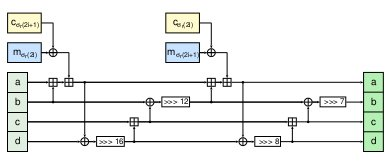
\includegraphics[width=4in]{blakeGfunction.jpg}
  \end{center}
  \caption{The $G_{i}$ function in BLAKE \cite{00002}}
  \label{fig:lab}
\end{figure}

\item {\bf Finalization:} The chaining values for the next stage are obtained by XOR of the words from the state 
matrix, the salt and the initial value.

$
h'_{0} \gets h_{0} \oplus s_{0} \oplus v_{0} \oplus v_{8} \\
h'_{1} \gets h_{1} \oplus s_{1} \oplus v_{1} \oplus v_{9} \\
h'_{2} \gets h_{2} \oplus s_{2} \oplus v_{2} \oplus v_{10} \\
h'_{3} \gets h_{3} \oplus s_{3} \oplus v_{3} \oplus v_{11} \\
h'_{4} \gets h_{4} \oplus s_{0} \oplus v_{4} \oplus v_{12} \\
h'_{5} \gets h_{5} \oplus s_{1} \oplus v_{5} \oplus v_{13} \\
h'_{6} \gets h_{6} \oplus s_{2} \oplus v_{6} \oplus v_{14} \\
h'_{7} \gets h_{7} \oplus s_{3} \oplus v_{7} \oplus v_{15} \\
$
\end{itemize}

{\bf Hashing the message}

A given input message is padded with a bit '1' followed followed by at most 511 bits of zeros, so that the message 
size is equal to 447 modulo 512. This padding is followed by a bit '1' and a 64-bit unsigned big-endian representation
of block length $l$. The padding to a message, can be represented as $m \gets m \parallel 1000 \dots 0001\langle l \rangle_{64}$

\begin{algorithm}
\caption{BLAKE Compression procedure \cite{00002}}
\begin{algorithmic}[1]
\State $ h^{0} \gets IV $
\For {$i = 0,\dots, N - 1$}
  \State $h^{i+1} \gets compress(h^{i}, m^{i}, s, l^{i})$
\EndFor
\State\Return{$h^{N}$}
\end{algorithmic}
\end{algorithm}

As shown in algorithm 1, the BLAKE compression function ingests the padded message block by block, in a loop 
starting from the initial value, and then sends the last chained value obtained from the finalization to the 
$\Omega$ truncation function, to obtain the hash value.

\subsubsection{ BLAKE-512 }
operates on 64-bit words and returns a 64-byte hash value. The chaining value is 512 bit long, message blocks are
1024 bits, salt is 256 bits, and counter size is 128 bits. The difference from BLAKE-256 are in constants compression 
function which gets 16 iterations, and the word size is of 64 bits. For the padding, the message is first padded with 
bit 1 and then as many zeros required to make the bit length equivalent to 895 modulo 1024. After that another bit of 
value 1 is appended followed by 128-bits unsigned big-endian representation of of message length

\subsection{Keccak}
Keccak hash function, is built on sponge construction, which can input and output arbitrary length strings. The sponge 
construction is used to build function $SPONGE[f, pad, r]$ which inputs and outputs variable length strings \cite{00016}. 
It uses fixed length permutation $f$, a padding "pad", and parameter bit rate 'r'. The permutations are operated on
fixed number of bits, width $b$. The value $c = b - r$ is the capacity of the sponge function. The width $b$ in Keccak
defines the state size which can be any of the following \{25, 50, 100, 200, 400, 800, 1600\} number of bits.

The $KECCAK-f[b]$ permutations are operated on state represented as a[5][5][w], with w = $2^{l}$, where l can be any value
from 0 to 6. The position in this 3 dimensional state is given by $a[x][y][z]$ where $x, y \in \mathbb{Z}_{5}$ and $z \in 
\mathbb{Z}_{w}$. The mapping of the bits from the input message 's' to state 'a' is like this $s[w (5y + x) + z] = a[x][y][z]$.
The $x, y$ coordinates are taken modulo 5, while the $z$ coordinate is taken as modulo $w$.  \cite{00015}

There are five steps, for a permutation round R.
\begin{center}R = $\zeta \circ \chi \circ \pi \circ \rho \circ \theta$. \end{center} 
These permutations are repeated for $12 + 2l$ times, with $l$ dependent on the variant chosen.

\begin{align*}
\theta &: a[x][y][z] & \gets & \thickspace a[x][y][z] + \displaystyle\sum\limits_{y' = 0}^{4} a[x - 1][y'][z] + \displaystyle\sum\limits_{y' = 0}^{4} a[x + 1][y'][z - 1], \\
\rho &: a[x][y][z] & \gets & \thickspace a[x][y][z - (t + 1)(t + 2) / 2], \\
& & & \thickspace t \thickspace satisfying \thickspace 0 \leq t < 24 \thickspace and \thickspace
\begin{pmatrix} 0 & 1 \\ 2 & 3 \end{pmatrix}^{t} \begin{pmatrix} 1 \\ 0 \end{pmatrix} = \begin{pmatrix} x \\ y \end{pmatrix}
in \thickspace GF(5)^{2 \times 2}, \\
& & & \thickspace or \thickspace t = -1 \thickspace if \thickspace x = y = 0, \\
\pi &: a[x][y] & \gets & \thickspace a[x'][y'], \thickspace with \thickspace
\begin{pmatrix} x \\ y \end{pmatrix} = \begin{pmatrix} 0 & 1 \\ 2 & 3 \end{pmatrix} \begin{pmatrix} x' \\ y'\end{pmatrix}, \\
\chi &: a[x] & \gets & \thickspace a[x] + (a[x + 1] + 1) \thickspace a[x + 2], \\
\zeta &: a & \gets & \thickspace a + RC[i_{r}].
\end{align*}

The addition and the multiplications are in Galois field GF(2), except for the round constants $RC[i_{r}]$. The round constants 
are given by

\begin{center} $RC[i_{r}][0][0][2^{j} - 1] = rc[j + 7i_{r}]$ for all $ 0 \leq j \leq l$, \end{center}

and the rest are zeros. The value of $rc[t] \in GF(2)$ is output of linear feedback shift register given as 

\begin{center}$rc[t] = (x^{t} \thickspace mod \thickspace x^{8} + x^{6} + x^{5} + x^{4} + 1)$ mod x in GF(2)[$x$].\end{center}

\section{Previous Work}

\subsection{Near collisions with Hill Climbing}

A generic algorithm applied to find near collisions, in reduced rounds of some SHA-3 competitors was hill climbing
\cite{00029}. Near collisions in which more than 75\% of the bits were same for two different messages, were found 
for reduced rounds of BLAKE-32, Hamsi-256 and JH. Near collision results are important for knowing the security
margins. In some cases, output of hash functions may be truncated for compatibility or efficiency purposes. In 
such cases near collisions could be improved to obtain collisions. A $\epsilon / n $ bit near collision for hash 
function h and two messages $M_{1}$ and $M_{2}$, where $M_{1} \neq M_{2}$ can be defined as
$HW( h( M_{1}, CV ) \oplus h( M_{2}, CV ) ) = n - \epsilon $ where HW is the Hamming weight, and CV is the chaining
value, and n is the hash size in bits.

The paper used hill climbing algorithm will be to minimize the function 

\begin{center}$f_{M_{1}, M_{2}}(x) = HW( h(M_{1}, x) \oplus h(M_{2}, x) )$\end{center}

where $x \in \{0, 1\}^{n}$, where $M_{1}$ and $M_{2}$ are message blocks. CV is chosen as any random chaining value.
The k-opt condition can be defined as 

\begin{center}k-opt = $f_{M_{1}, M_{2}} (CV) =  \min\limits_{x \in S^{k}_{CV}} f_{M_{1}, M_{2}} (x)$\end{center}

\begin{algorithm}
  \caption{ Hill Climbing Algorithm ($M_{1}, M_{2}, k$) for near collisions }
  \begin{algorithmic}[1]
    \State Randomly select $CV$
    \State $f_{best} = f_{M_{1}, M_{2}}(CV)$
    \State \While {($CV$ is not k-opt)}
    \State $CV$ = $x$ such that $x \in S^{k}_{CV}$ with $f(x) < f(best)$
    \State $f_{best} = f_{M_{1}, M_{2}}(CV)$
    \State \EndWhile
    \State \Return ($CV$, $f_{best}$)
  \end{algorithmic}
\end{algorithm}

Algorithm 2, shows how hill climbing is used to obtain near collisions. Given two message $M_{1} \thickspace and \thickspace M_{2}$, 
and a randomly chosen chaining value CV, the $f_{M_{1}, M_{2}}(CV)$ is obtained. The set $S^{k}_{CV}$ is searched
for a better fit CV, and if found is updated. And the search is repeated again in the k-bit neighbourhood of new CV.

\subsection{Simulated Annealing}

\begin{algorithm}
  \caption{ Simulated Annealing Algorithm for obtaining near collisions }
  \begin{algorithmic}[1]
    \Function {Simulated-annealing}{$M_{1}, M_{2}, CV,$ schedule}
      \State current $\gets \thickspace CV$
      \For { t = 1 to $\infty$ }
        \State T $\gets$ schedule( t )
        \If { T = 0}
          \State \Return current
        \EndIf
        \State next $\gets$ a randomly selected successor from set $S^{k}_{current}$
        \State $\Delta E \gets  \thickspace f_{M_{1}, M_{2}}(current) - f_{M_{1}, M_{2}}(next)$
        \If { $\Delta$E $>$ 0 }
          \State current $\gets$ next
        \Else
          \State current $\gets$ next, with probability $e^{\Delta E / T}$
        \EndIf
      \EndFor
    \EndFunction
  \end{algorithmic}
\end{algorithm}

The problem with hill climbing, is that it can get locked in the local maxima, and fail to get the global maxima.
This is due to hill climbing not taking a downhill or a step with lower value. However, if hill climbing is 
tweaked to combine with random walk, then the problem of local maxima can be avoided. Simulated annealing picks
a random successor, and accepts it if the value is higher than previous. However, if the successor has a lower
value, then it is accepted with a probability less than 1. The probability has an exponential decrease proportional
to the decreased value of the move, and the temperature. Thus at higher temperature or at the initial stages, a
downhill successor is more likely to be accepted, than in the later stages \cite{00033}.

\subsection{Tabu Search}

\begin{algorithm}[h]
  \caption{ Tabu Search for obtaining near collisions \cite{00036}}
  \begin{algorithmic}[1]
    \Function {Tabu-search}{$TabuList_{size}, M_{1}, M_{2}, CV$}
      \State $S_{best}$ $\gets \thickspace CV$
      \State $TabuList \thickspace \gets$ null
      \While {$S_{best}$ not k-opt}
        \State CandidateList $\gets$ null
        \State $S_{neighbourhood} \gets S^{k}_{S_{best}}$
        \For { $S_{candidate} \in S_{best_{neighbourhood}}$}
          \If {not ContainsAnyFeatures( $S_{candidate}, TabuList$ )} 
            \State CandidateList $\gets$ $S_{candidate}$
          \EndIf
        \EndFor
        \State $S_{candidate}$ $\gets$ LocateBestCandidate( CandidateList )
        \If { Cost( $S_{candidate}$ ) $\leq$ Cost( $S_{best}$ ) }
          \While { $TabuList >TabuList_{size}$ }
            \State DeleteFeature( $TabuList$ )
          \EndWhile
        \EndIf
      \EndWhile 
      \State \Return $S_{best}$
    \EndFunction
  \end{algorithmic}
\end{algorithm}

Tabu search implements the neighbourhood search for the solutions, until the termination condition. The algorithm
uses a fixed amount of memory, to keep note of states, visited some fixed amount of time in past. The idea behind
keeping the state, is to restrict the search, to states that have not been visited previously. The algorithm can be
tweaked, to accept moves in tabu list through aspiration criteria, or inferior moves just to explore new possible
states. Tabu search has been applied to mostly combinatorial optimization problems\cite{ 00034, 00035 }.

\section{Methodology}

\subsection{Design of Experiment}
I aim to use hill climbing, simulated annealing, tabu search, random selection algorithms, to search for near 
collisions, for two chosen message $M_{1},M_{2}$ where $M_{1} \neq M_{2}$. This will be done as shown by implementing
the algorithms 2, 3, 4 and 5.

\begin{algorithm}[h]
  \caption{ Random selection from k-bit neighbourhood of $CV$ }
  \begin{algorithmic}[1]
    \Function {Random-Selection}{$ M_{1}, M_{2}, CV,$ number\_of\_trials}
      \State current $\gets \thickspace CV$
      \State trial $\gets$ 0
      \While { trial $<$ number\_of\_trials }
        \State next $\gets$ randomly selected candidate from $S^{k}_{current}$
        \If { $f_{M_{1}, M_{2}}(next) - f_{M_{1}, M_{2}}(current) $ }
          \State current $\gets$ next
        \EndIf
      \EndWhile 
      \State \Return current
    \EndFunction
  \end{algorithmic}
\end{algorithm}

  \subsubsection{Data}
  
  For creating the message pair, I intend to choose the first message as "The quick brown fox jumps over the lazy dog.".
  Another 14 messages will be created from the initial message, so in all we get %$\begin{pmatrix} 15 \\ 2 \end{pmatrix} = 105$
  105 pairs of message in total. The rest of the 14 messages will be derived from the first message by applying a
  shift register operation, that results in a bit flip from the previous message. For example, if my initial message has
  a bit pattern of 0000. Then the subsequent messages will be 1000, 1100, 1110 and 1111.
  
  This will give the experiment an advantage of comparing substantial message pairs with small to medium Hamming distance.
  The initial chaining value for experiment is chosen randomly, and does not matter as long it is kept constant provided
  to all the message pairs in the experiment. I intend to use the hash value of empty string generated by Keccak as the 
  initial chaining value for all the pairs.

  \subsubsection{Procedure}

  Both Keccak and Gr{\o}stl can support variable byte message digest length, but BLAKE based on SHA-2 designs can have
  message digests of 224, 256, 384 and 512 bits. Thus the experiment for 105 pairs will be done on 4 message sizes as
  indicated by BLAKE. Keccak does not have a initial state or a chaining value as such, but can be tweaked, so that it
  has the first sponge state to accept the chaining value and pre-compute it and then apply the hash function on the
  message.

  Reduced state for the hash functions can be obtained, by either reducing the number of rounds the permutations
  are executed, or by reducing the number of bits in the internal state of the hash function.

\subsection{Platform, Architecture, Languages and Tools}
The platform I would most likely choose will be Ubuntu 12.04 LTS, with the primary coding language
being \href{"https://en.wikipedia.org/wiki/Java\_(programming_language)"}{Java} or 
\href{"http://golang.org/"}{Go-lang}.The initial data that needs to be calculated for all the pairs 
of message will be static for the rest of the experiment,and stored for rest of the experiment.

The first task will be creation of the data. First, pairs of initial message will have to be 
made. Each of the message from the pair will be line separated, and each of the pair in the file
will be separated with a blank line. This will be the initial data file. All the three hash functions
will be implemented and then tested against the existing implementations, for correctness. These
implemented hash function, will then be used for the experimentation with reduced rounds. In order
to conduct the experiment smoothly, a graphical user interface (GUI) window will be created, with
various parameters for the digest size, internal state size, message pairs, number of trials etc.
This GUI will control the experimental setup and execute the test cases on hash functions and dump
the results as required.

The output for the results will be stored in the following format. The directory structure for the
output will be algorithm name, followed by digest size. Followed by algorithm name whose digest 
pairs are being examined. Followed by the file name for that particular message pair. For this message 
I intend to create 15 messages, and they can be named from A to O. Thus a pairing of first message to 
second message will make the output file name to be AB.txt. So when the simulated annealing algorithm 
evaluates the hash values pairs of Keccak algorithm with digest size of 512 bits, and for message pair.
Then the output will be stored in directory hierarchy as simulated\_annealing/512/Keccak/AB.txt.

The output file will be organised in same way as the input files, with each data line separated, and 
each experiment data separated by a blank line. The output for each experiment in hill climbing will
have the bit representation of the XOR value of two message digests, along with the chaining value
that was last obtained and the time taken for that experiment.

\subsection{Proposed Schedule}
\begin{table}[h]
  \begin{center}
    \begin{tabular}{ | p{12cm} | c | } \hline
      Tasks                                                                                                   & Timeline \\ \hline
      Project proposal Approved. Completing 3rd party cryptanalysis part of report for Keccak.                & July 26 \\ \hline
      Creation of message pairs and coding 2 hash functions. Write cryptanalysis part for BLAKE in report.    & August 2 \\ \hline
      Coding the 3rd hash function, validation testing, finishing cryptanalysis part for Gr{\o}stl in report. & August 9 \\ \hline
      Code and test the hill climbing algorithm, and start collecting data from output.                       & August 16 \\ \hline
      Run experiments, collect more data, and put them in report. Discuss the results with advisor.           & August 23 \\ \hline
      Fine tune the experiment, collect data and start writing observations and conclusion part in report.    & August 30 \\ \hline
      Discuss results and conclusions with advisor. Fine tune report. Run more experiments if required.       & September 6 \\ \hline
      Format the report properly, and submit it for acceptance. Create presentation for project defense.      & September 13 \\ \hline
      Check availability of faculty. Announce defense date, book room and defend by September 20              & October 11 \\ \hline
    \end{tabular}
  \caption{Proposed schedule for my project implementation.}
  \end{center}
\end{table}

\section{Evaluation and expected outcomes}
The experiment with each of the pair, will be run for approximately $2^{10}$ times or rather 1024 times.
The attacks will be done on both full and reduced versions of hash functions.The following are the parameters
on which I propose to evaluate the algorithms. 

\begin{enumerate}
  \item How much time for each of the respective message digest size, did it take for the simulated
  annealing, tabu search, hill climbing and random selection, to find a near collision.
  \item How much is the Hamming distance on an average for the chaining value that is manipulated by
  search algorithms for each of the hash functions.
  \item Till how many rounds, is the each of the search algorithm a feasible option to find near 
  collisions, for each of the hash function.
  \item Is the weight of the Hamming distance between message pair co-related to the amount of work
  for each of the search algorithm does to find a collision.
  \item Does the Hamming weight distance between message pair, vary for each of the hashing algorithm
  with respect to amount of work on average required by search algorithm.
  \item On an average what was the hamming distance of the chaining value obtained from a successful
  experiment from the individual message.
  \item On an average, which of the attack algorithms is most likely to find a near collision.
  \item Statistical analysis will be carried on the data collected for t-tests, $\chi^{2}$ tests,
  confidence interval etc, to make concrete claims.
\end{enumerate}

The above list is tentative, and by no means exhaustive. If during the course of experiment, more 
interesting figures come in front, then they will be added.

\bibliographystyle{plain}
\bibliography{CapstoneBib}

\end{document}
